% --- Historical arc and vision FM taxonomy ---
\begin{frame}{2012: Deep learning emerges in AI}
  \centering
  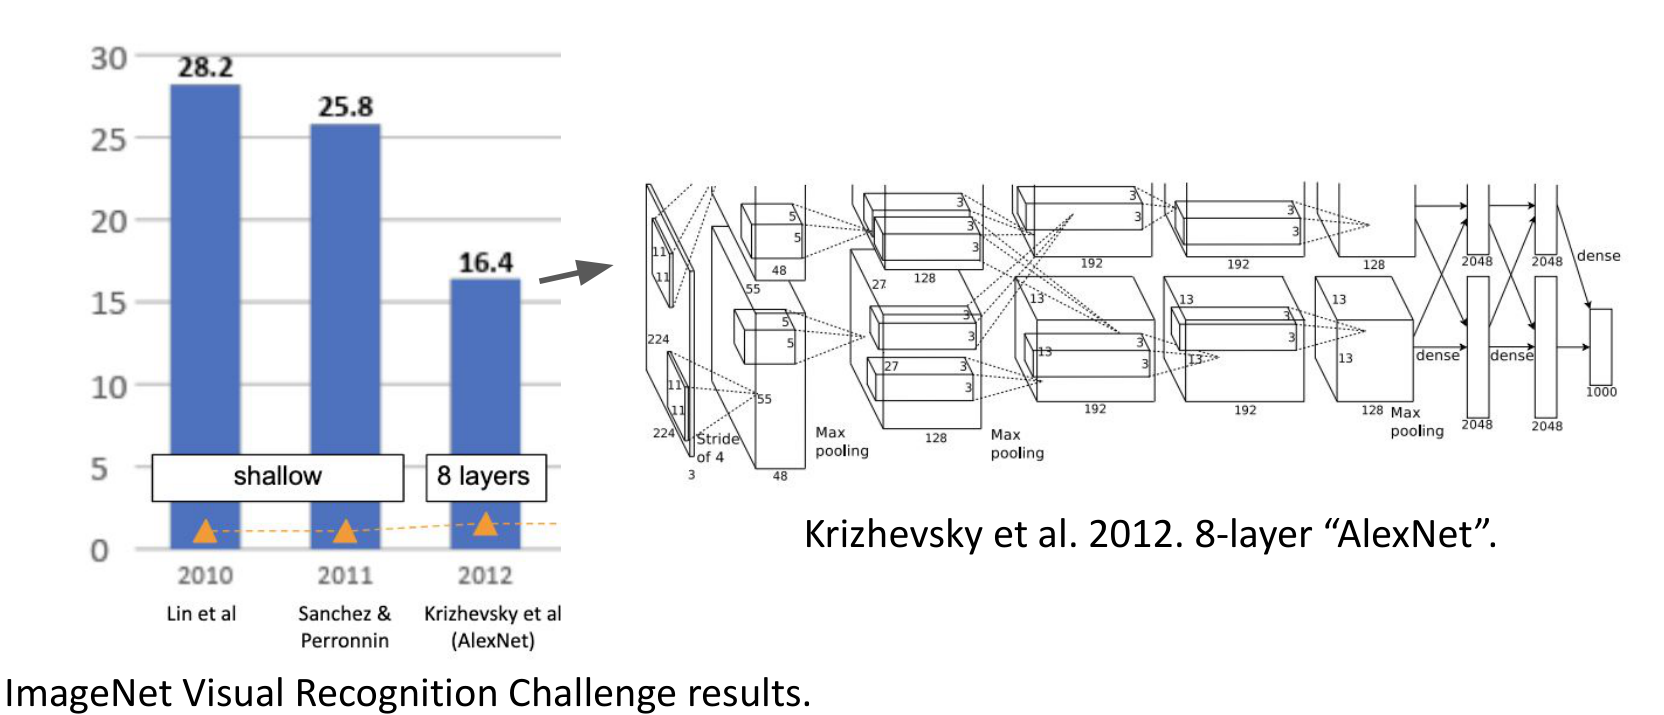
\includegraphics[width=\textwidth,height=0.86\textheight,keepaspectratio]{images/foundation-models/imagenet_challenge_alexnet.png}
\end{frame}

\begin{frame}{Convergence of key ingredients of deep learning}
  \centering
  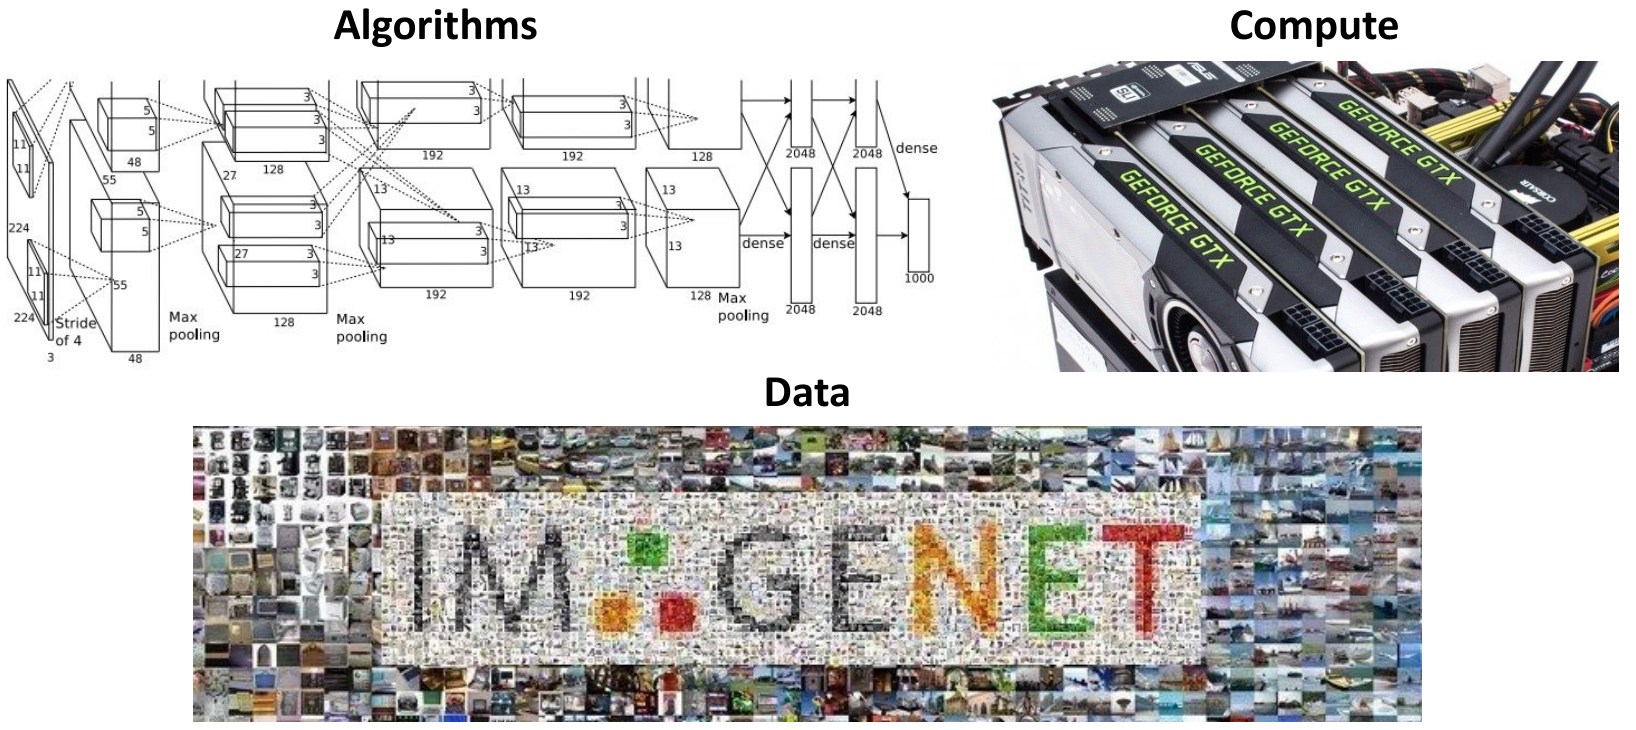
\includegraphics[width=\textwidth,height=0.86\textheight,keepaspectratio]{images/foundation-models/imagenet_algorithms_compute_data.png}
\end{frame}

\begin{frame}{2015: Very deep convnets and challenging vision tasks}
  \centering
  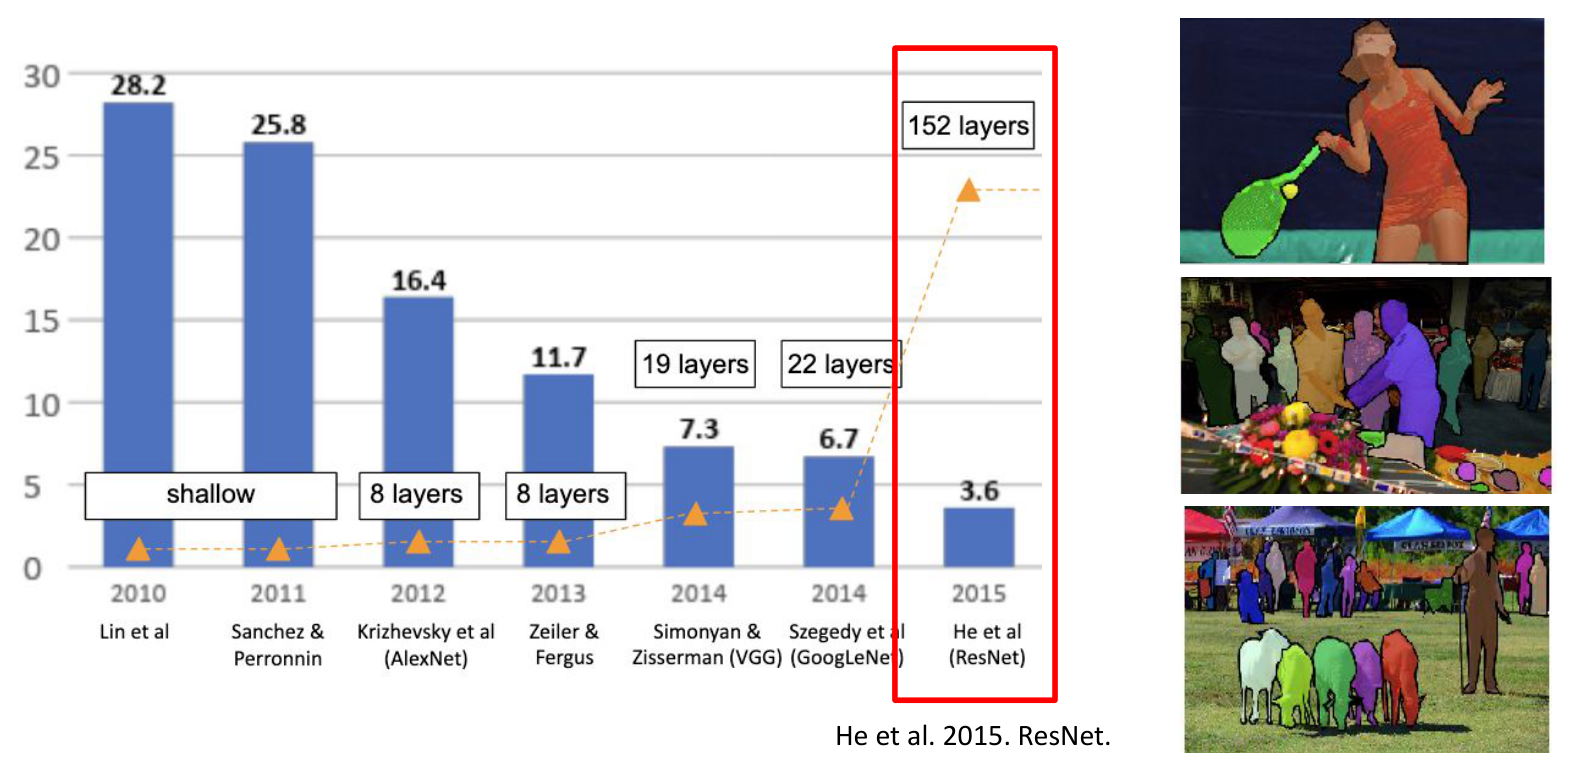
\includegraphics[width=\textwidth,height=0.86\textheight,keepaspectratio]{images/foundation-models/imagenet_depth_progression_resnet.png}
\end{frame}

\begin{frame}{2018: Breakthroughs in deep learning for natural
  language processing (sequences)}
  \centering
  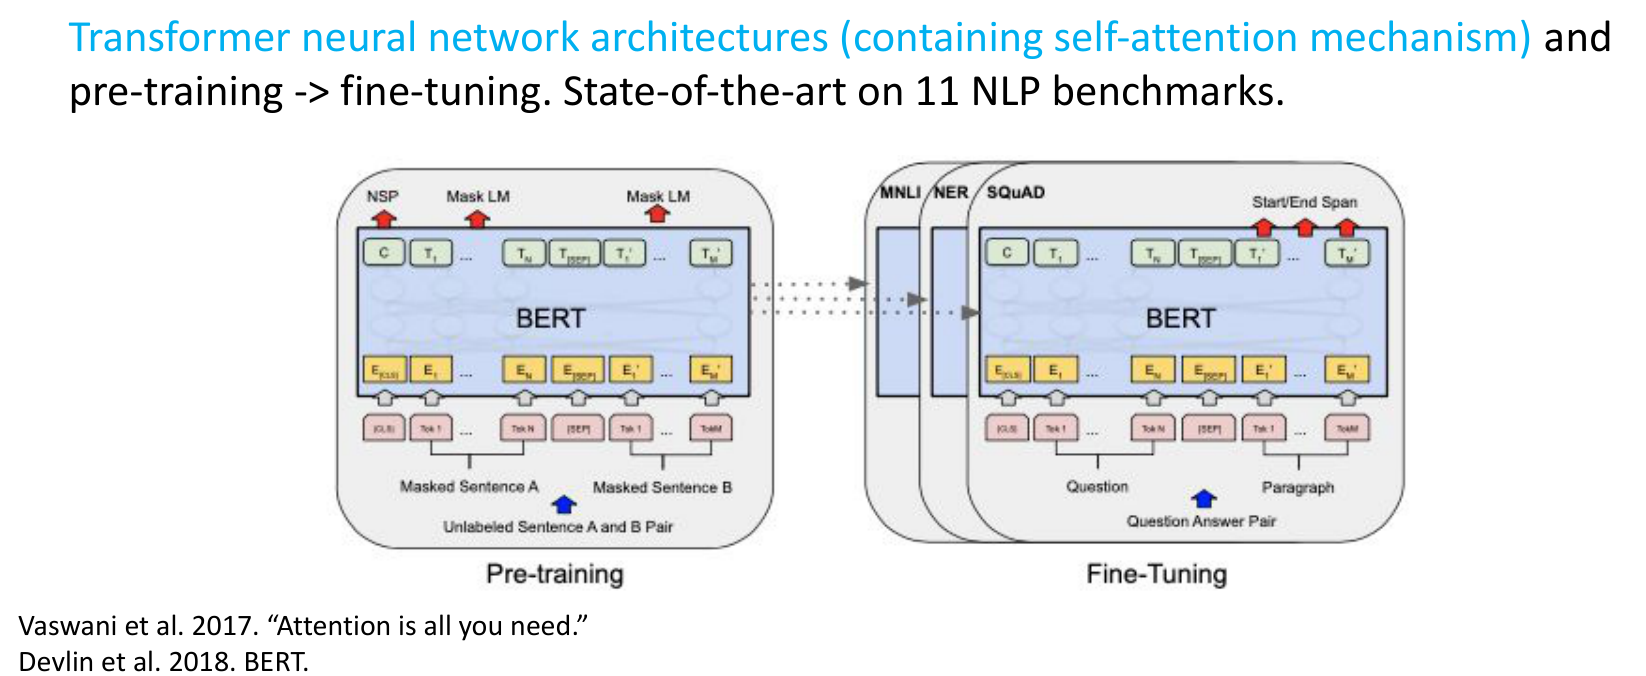
\includegraphics[width=\textwidth,height=0.86\textheight,keepaspectratio]{images/foundation-models/bert_pretraining_finetuning.png}
\end{frame}

\begin{frame}{2020: Very large-scale text generation models}
  \centering
  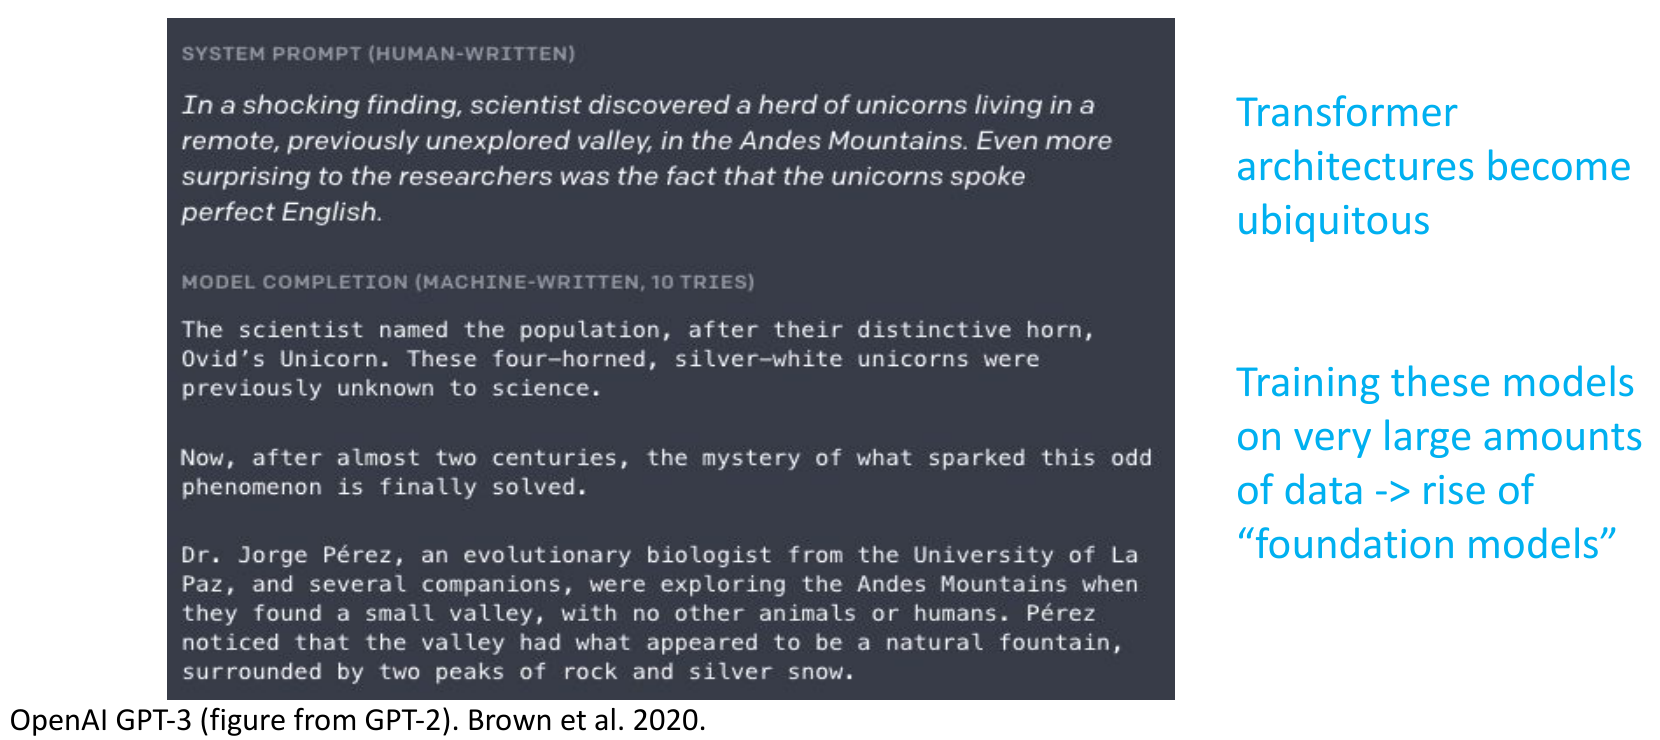
\includegraphics[width=\textwidth,height=0.86\textheight,keepaspectratio]{images/foundation-models/gpt3_unicorns_foundation_models.png}
\end{frame}

\begin{frame}{2021: Transformers & foundation models reach computer vision}
  \centering
  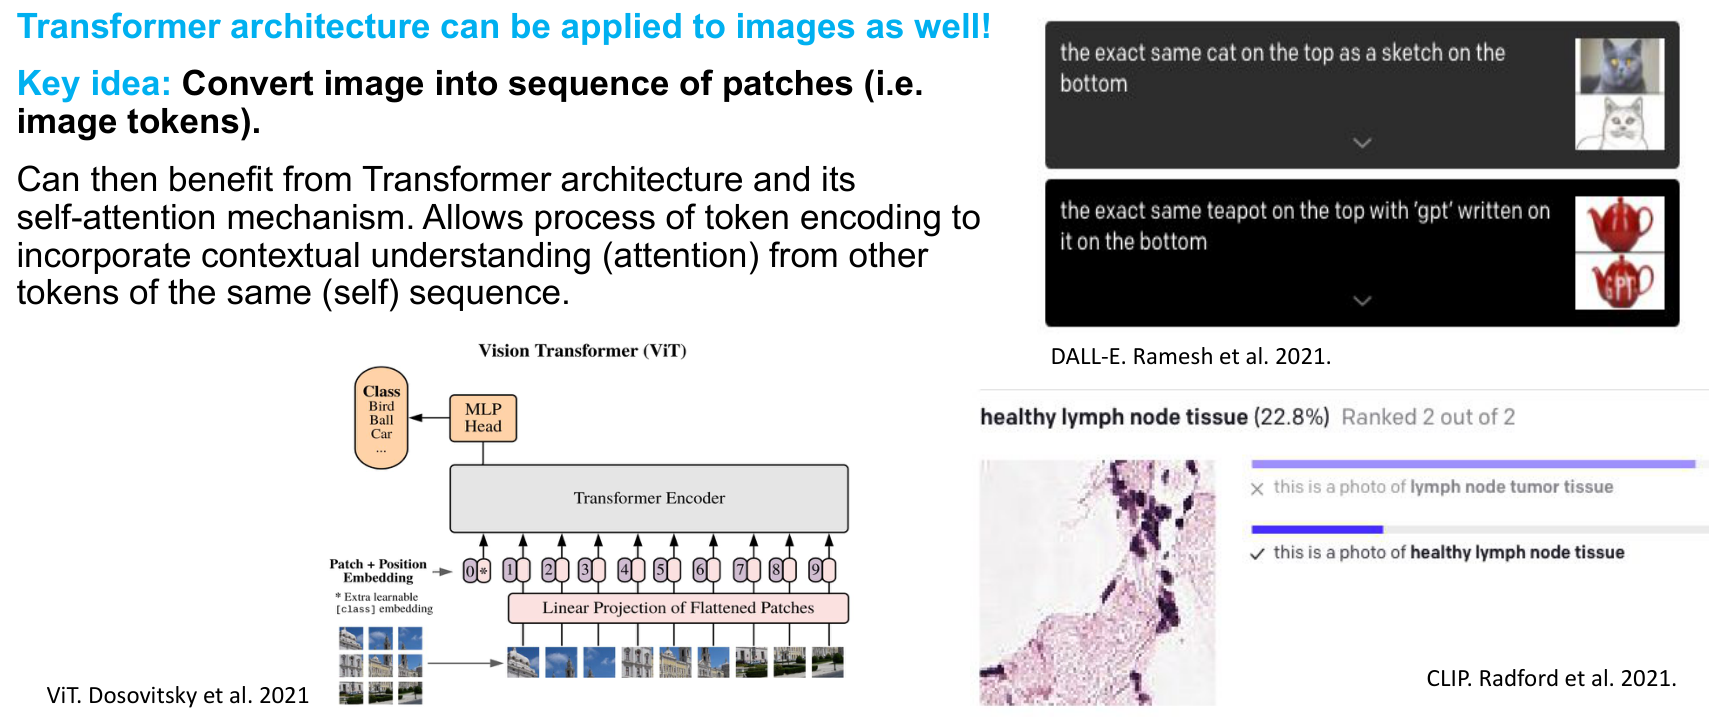
\includegraphics[width=\textwidth,height=0.86\textheight,keepaspectratio]{images/foundation-models/vit_vision_transformer_patches.png}
\end{frame}

\begin{frame}{2022: Major improvements in text-to-image generation models}
  \centering
  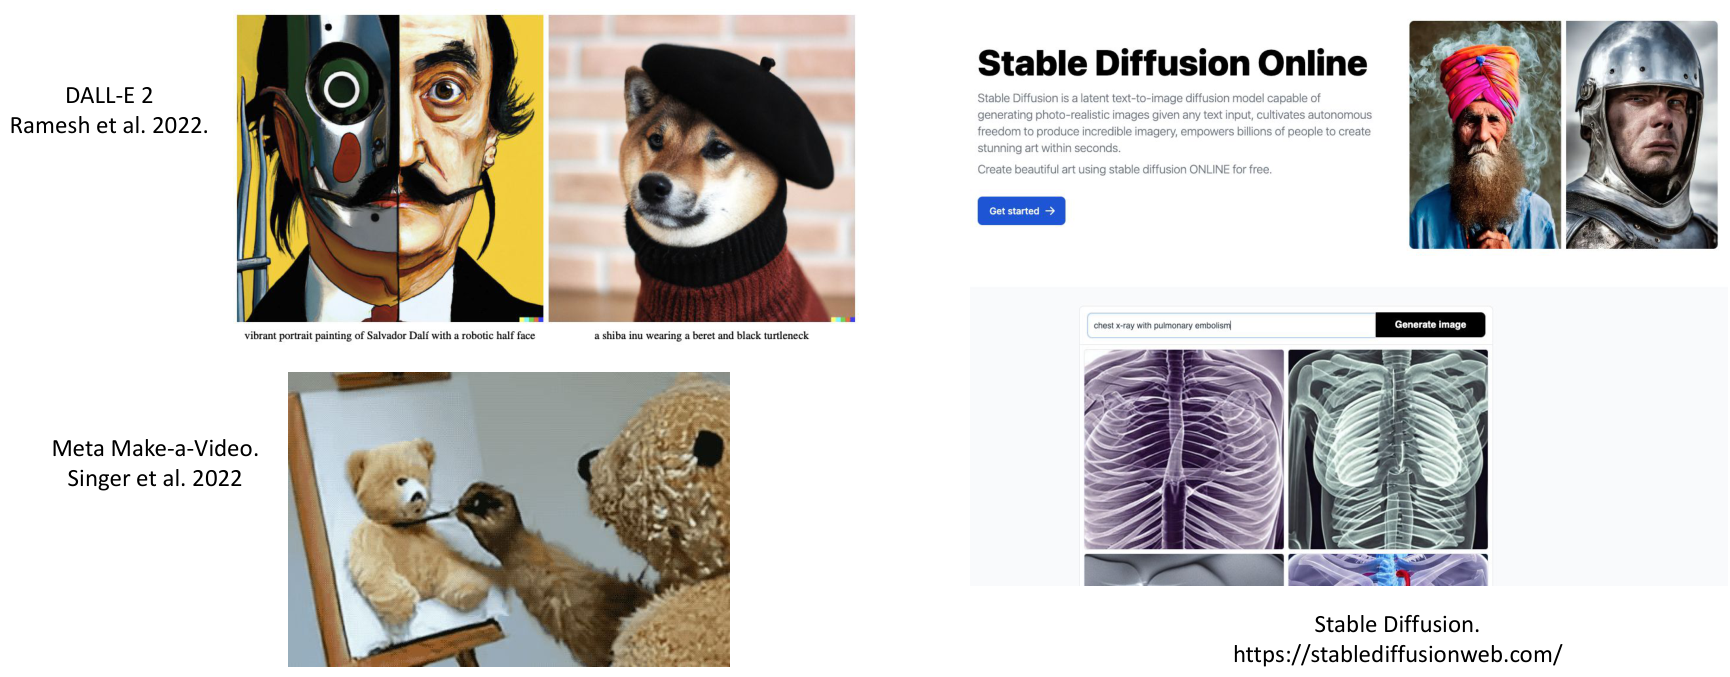
\includegraphics[width=\textwidth,height=0.86\textheight,keepaspectratio]{images/foundation-models/generative_dalle_stable_diffusion.png}
\end{frame}

\begin{frame}{Late 2022: ChatGPT reaches public mainstream}
  \centering
  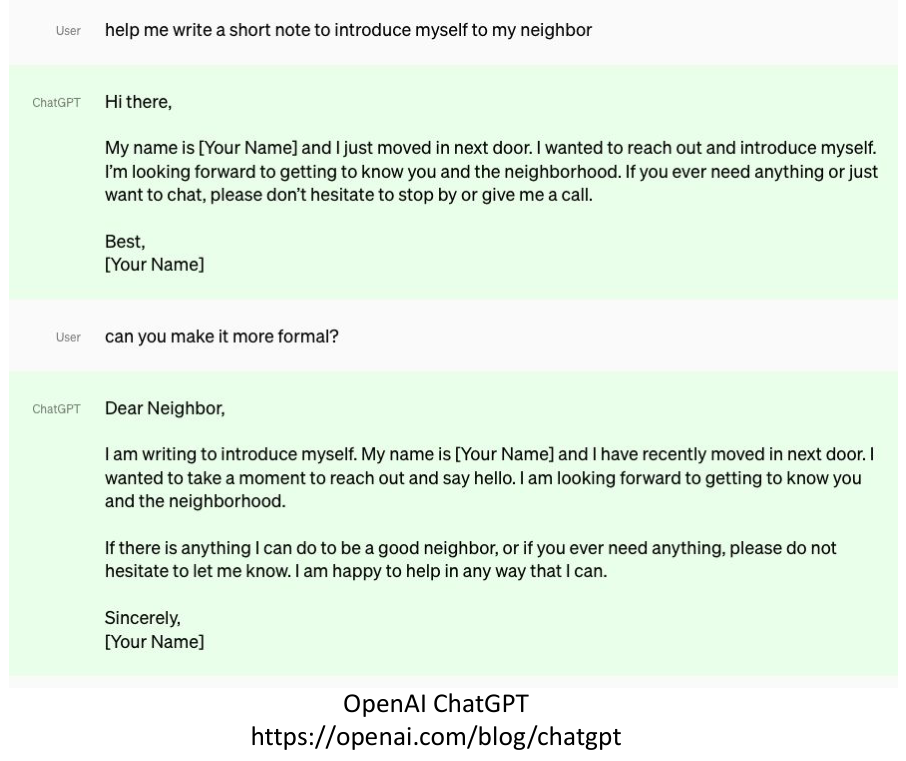
\includegraphics[width=\textwidth,height=0.86\textheight,keepaspectratio]{images/foundation-models/chatgpt_example_conversation.png}
\end{frame}


\begin{frame}{Two major classes of vision foundation models}
  \begin{columns}[T,onlytextwidth]
    \column{0.48\textwidth}
      {\color{KAUSTblue}\textbf{Representation Learners}} \\[0.5em]
      {\color{KAUSTred}Train on huge amounts of data} \\[0.2em]
      \textbf{Objective:} learn powerful generalist feature extractors that can be used for downstream computer vision tasks.
      \begin{itemize}\itemsep0.32em
        \item Vision Only (e.g.\ DINOv2)
        \item Vision-Language (e.g.\ CLIP)
      \end{itemize}
    \column{0.04\textwidth}
    \column{0.48\textwidth}
      {\color{KAUSTcyan}\textbf{Generative Models}} \\[0.5em]
      {\color{KAUSTred}Train on huge amounts of data} \\[0.2em]
      \textbf{Objective:} learn to generate images and/or text.
      \begin{itemize}\itemsep0.32em
        \item Text $\rightarrow$ Image (e.g.\ Stable Diffusion, DALL-E)
        \item Text, Image $\rightarrow$ Text (e.g.\ Flamingo, GPT4-V)
      \end{itemize}
  \end{columns}
\end{frame}
